% !TEX encoding = UTF-8 Unicode
\documentclass[a4paper]{article}

\usepackage{color}
\usepackage{url}
\usepackage[T2A]{fontenc} % enable Cyrillic fonts
\usepackage[utf8]{inputenc} % make weird characters work
\usepackage{graphicx}

\usepackage[english,serbian]{babel}

\usepackage[unicode]{hyperref}
\hypersetup{colorlinks,citecolor=green,filecolor=green,linkcolor=blue,urlcolor=blue}

\usepackage{listings}

\definecolor{mygreen}{rgb}{0,0.6,0}
\definecolor{mygray}{rgb}{0.5,0.5,0.5}
\definecolor{mymauve}{rgb}{0.58,0,0.82}

\lstset{ 
  backgroundcolor=\color{white},   % choose the background color; you must add \usepackage{color} or \usepackage{xcolor}; should come as last argument
  basicstyle=\footnotesize,        % the size of the fonts that are used for the code
  breakatwhitespace=false,         % sets if automatic breaks should only happen at whitespace
  breaklines=true,                 % sets automatic line breaking
  captionpos=b,                    % sets the caption-position to bottom
  commentstyle=\color{mygreen},    % comment style
  deletekeywords={...},            % if you want to delete keywords from the given language
  escapeinside={\%*}{*)},          % if you want to add LaTeX within your code
  extendedchars=true,              % lets you use non-ASCII characters; for 8-bits encodings only, does not work with UTF-8
  firstnumber=1000,                % start line enumeration with line 1000
  frame=single,	                   % adds a frame around the code
  keepspaces=true,                 % keeps spaces in text, useful for keeping indentation of code (possibly needs columns=flexible)
  keywordstyle=\color{blue},       % keyword style
  language=Python,                 % the language of the code
  morekeywords={*,...},            % if you want to add more keywords to the set
  numbers=left,                    % where to put the line-numbers; possible values are (none, left, right)
  numbersep=5pt,                   % how far the line-numbers are from the code
  numberstyle=\tiny\color{mygray}, % the style that is used for the line-numbers
  rulecolor=\color{black},         % if not set, the frame-color may be changed on line-breaks within not-black text (e.g. comments (green here))
  showspaces=false,                % show spaces everywhere adding particular underscores; it overrides 'showstringspaces'
  showstringspaces=false,          % underline spaces within strings only
  showtabs=false,                  % show tabs within strings adding particular underscores
  stepnumber=2,                    % the step between two line-numbers. If it's 1, each line will be numbered
  stringstyle=\color{mymauve},     % string literal style
  tabsize=2,	                   % sets default tabsize to 2 spaces
  title=\lstname                   % show the filename of files included with \lstinputlisting; also try caption instead of title
}

\begin{document}

\title{Programski jezik Objective-C\\ 
\small{Seminarski rad u okviru kursa\\Metodologija stručnog i naučnog rada\\ Matematički fakultet}}

\author{Dalma Beara, Denis Aličić, Mateja Marjanović, Anja Miletić
\\beara.dalma@gmail.com, a.denis96@gmail.com,\\ mateja.marjanovic96@gmail.com, anya.miletic@gmail.com}

\maketitle

\abstract{
U ovom radu je opisan nastanak i razvoj programskog jezika Objective-C, kao i njegova uloga u razvoju drugih jezika koji imaju široku primenu(Java, Swift) kao i bitnih koncepata koji su počevši od Objective-C ušli u upotrebu (interfejsi). Predstavljene su osnovne karakteristike jezika i najbitniji koncepti koje jezik, na kom je zasnovan operativni sistem MAC OS, implementira kao i najpoznatija razvojna okruženja (eng.~{\em framework}).   

\setcounter{tocdepth}{1}
\tableofcontents

\newpage

\section{Uvod}
\label{sec:uvod}
Objective-C je objektno-orijentisan programski jezik namenjen kako za sistemsko programiranje, tako i za izradu korisničkih aplikacija. Nastao iz potrebe za većom produktivnosti programera.
Kroz naredna poglavlja biće predstavljen uticaj jezika na svet kakav danas poznajemo kao i primeri u kojima je korišćen Objective-C za implementaciju čitavih operativnih sistema i korisničkih okruženja.  

\section{Nastanak i istorijski razvoj, mesto u razvojnom stablu, uticaji drugih programskih jezika}
\label{sec:osnovno}

\subsection{Nastanak i istorijski razvoj}
\label{subsec:istorija}
Iako se pojam jezika Objective-C primarno vezuje za proizvode kompanije Epl (engl. Apple) -- MAC OS X, iPhone itd, on je zapravo nastao mnogo pre njih. Njegove temelje postavili su Bred Koks i Tom Lav 1981. godine, težeći da nađu način za povećavanje produktivnosti programera. Te godine pojavio se novi, revolucionarni jezik Smalltalk \cite{smalltalk}, koji je tada unapredio koncept objektno-orijentisanog programiranja. U osnovi tog jezika bilo je posmatranje programa kao skupova objekata koji su mogli da komuniciraju jedni sa drugima dinamički pozivajući metode. To je omogućilo da se stanje programa menja pod uticajem korisnika. Koks je u ovoj ideji video mogućnost da se vrtoglavo ubrza pisanje programa, pošto su se u njemu mogle praviti biblioteke objekata i posle koristiti u drugim programima bez izmene. Međutim, Smalltalk je bio veoma spor i zahtevao je da se svi programi pišu i pokreću u posebnom okruženju. Tada se javila potreba za spajanjem objektno-orijentisanih ideja Smalltalk-a i brzog jezika C. Koks je 1983. objavio naučni rad u kom je predstavio objektno-orijentisani prekompilator (eng.~{\em Object-Oriented Precompiler}). Da bi ovu svoju ideju izbacili na tržište, njih dvojica su osnovali kompaniju Stepstoun (eng.~{\em Stepstone}), izmenili kompilator za OOPC i preimenovali jezik u Objective-C. Iako je glavna ideja ovog projekta bila pisanje i prodavanje pomenutih biblioteka koje su mogle ponovo da se koriste, korisnici su imali dosta zamerki, te je jezik sve više poprimao karakteristike objektno-orijentisanih jezika kakve ih danas znamo, kao što su sakupljač otpada (eng.~{\em garbage collector}) i interpreter, te je kompanija uskoro propala. Stiv Džobs je 1988. kupio licencu, a nekoliko godina kasnije i sva prava za Objective-C za potrebe svoje kompanije NeXT Computer koja se  1996. pripojila Apple-u. Sa tom tranzicijom, sam jezik je pretrpeo razne promene, a najvažnije su uvođenje dveju novih ,,komponenti'': kategorija (eng.~{\em categories}), danas poznatih kao ekstenzije (eng.~{\em extensions}) i protokola (eng.~{\em protocols}). Kategorije su služile da programerima omoguće da sami dodaju funkcije u objekte iz već postojećih biblioteka, a protokoli su omogućavali objektima da komuniciraju jedni s drugima. Oni su danas podržani u jeziku Java i poznati su kao interfejsi (eng.~{\em interfaces}). 

\begin{table}[h!]
\begin{center}
\begin{tabular}{|c|c|} \hline
jezik &preuzeto \\ \hline
C &imperativni koncepti \\ \hline
Smalltalk &objektno-orijentisani koncepti \\ \hline
\end{tabular}
\label{tab:tabela1}
\end{center}
\end{table}

Najpopularniji jezici na koje je uticao Objective-C su Swift i Java, a navode se još i Groovy, TOM, Nu i Objective-J.

\begin{figure}[h!]
	\begin{center}
	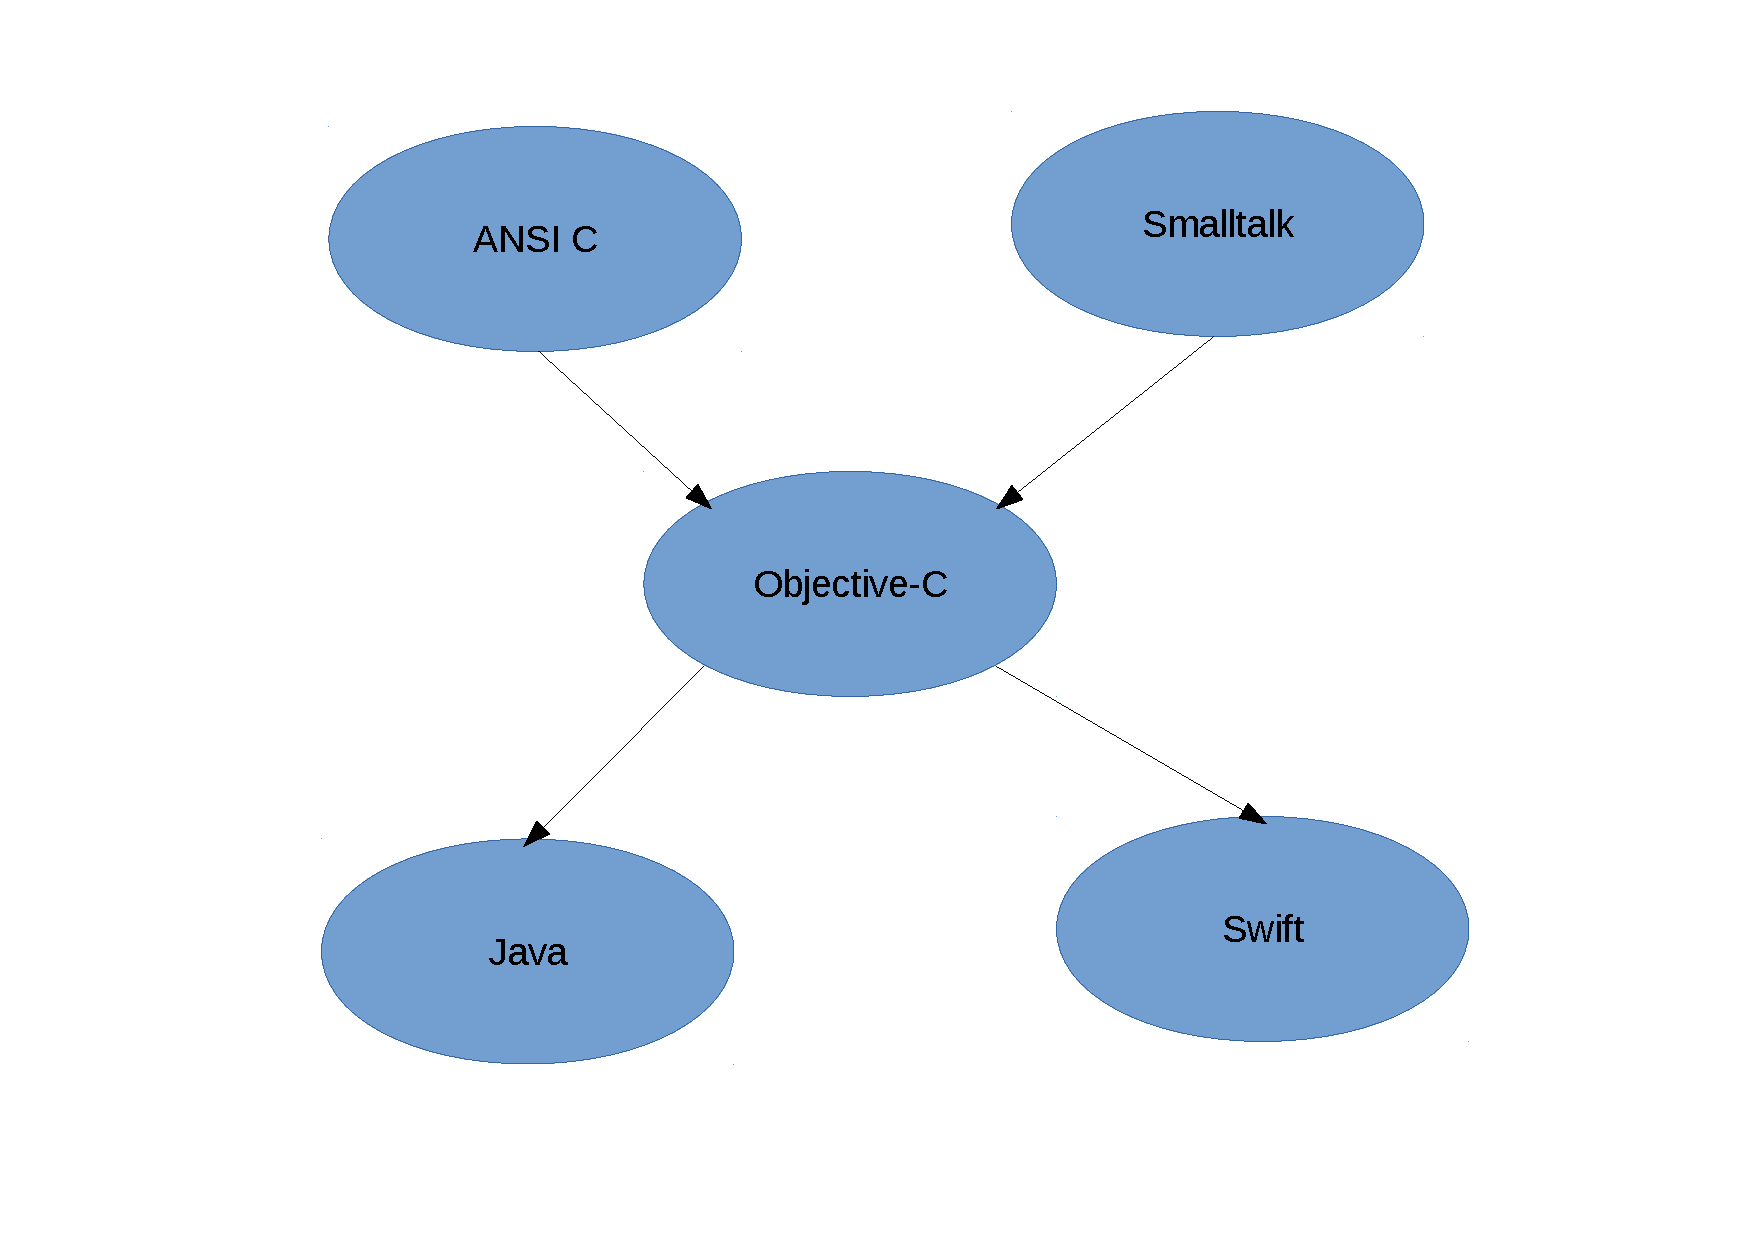
\includegraphics[scale=0.4]{razvojno_stablo.pdf}
	\caption{Razvojno stablo}	
	\label{fig:Razvojno_stablo}
	\end{center}
\end{figure}

\subsection{Uticaj drugih programskih jezika}
\label{subsec:uticaj}
Kao što je već navedeno, Objective-C je nastao kao kombinacija koncepata na kojima počiva Smalltalk utočenih u sintaksu jezika C. Isprva je čak funkcionisao tako što je kod prevođen na C i onda izvršavan. S druge strane, on je uticao na jezik Swift koji je razvio Epl. Swift \cite{swift} se često naziva i ,,Objective-C bez C-a'' kao i na Javu \ref{fig:Razvojno_stablo}. 

\section{Osnovna namena programskog jezika, svrha i mogućnosti}
\label{sec:namena}
Krajem 80-ih godina prošlog veka, popularnost Objective-C jezika je rasla sa razvojem NeXT sistema. Najviše se koristi za razvoj softvera za Apple iOS operativni sistem. Uticaj Objective-C jezika je vidljiv u Java programskom jeziku.
Objective-C definiše mali ali moćan skup ekstenzija ANSI C programskog jezika koje omogućavaju objektno-orijentisano programiranje. Cocoa \ref{sec:Cocoa}, Apple-ov API za macOS je napisan uz pomoć Objective-C jezika, takodje veliki deo aplikacija je napisan koristeći taj jezik. 

\section{Osnovne osobine ovog programskog jezika, podržane paradigme i koncepti}
\label{sec:osobine}
Objective-C je nadskup C programskog jezika koji pruža objektno-orijentisane sposobnosti i dinamičko izvršno okruženje (eng.~{\em runtime}). Objective-C nasledjuje sintaksu, primitivne tipove i naredbe za tok izvršavanja od jezika C, a dodaje sintaksu za definisanje klasa i metoda. Takodje omogućava dinamičko tipiziranje i povezivanje.
\subsection{Osnovni koncepti}
\subsubsection{Klasteri klasa}
Klasteri klasa (eng.~{\em class clusters}) su programski šablon koji se često koristi u pisanju programa na Objective-C jeziku. Klasteri klasa grupišu odredjeni broj privatnih podklasa unutar javne apstraktne nadklase. 
Ovakvo grupisanje pojednostavljuje javno vidljivu arhitekturu objektno-orijentisanih biblioteka i radnih okvira, bez smanjenja njihove funkcionalnosti. Apstraktna nadklasa mora da deklariše metode za kreiranje instanci svojih privatnih podklasa. 
\subsubsection{Introspekcija}
Introspekcija je moćno svojstvo objektno-orijentisanih jezika i okruženja. Ono predstavlja mogućnost objekta da predstavi detalje o sopstvenoj implementaciji u toku izvršavanja programa. Ti detalji mogu biti njegovo mesto u drvetu nasledjivanja, da li implementira odredjeni protokol i da li odgovara na neku poruku. Primer: 
\begin{lstlisting}[frame=single]
while ( id anObject = [objectEnumerator nextObject] ) {
    if ( [self class] == [anObject superclass] ) {
        // do something appropriate...
    }
}
\end{lstlisting}
\subsubsection{Alokacija objekata}
Prilikom alokacije objekata, dodeljuje se zahtevana memorija iz regiona virtualne memorije dostupne programu. Da bi se izračunalo koliko memorije treba alocirati, uzimaju se u obzir instancirane promenjlive tog objekta - uključujući njihove tipove i redosled - kao što je navedeno u klasi objekta.

\subsubsection{MVC}
MVC (eng.~{\em Model-View-Controller}) je programski šablon (eng.~{\em design pattern}) visokog nivoa koji predstavlja globalnu arhitekturu aplikacije i razvrstava objekte prema ulozi koju imaju u toj aplikaciji.
Objektno-orijentisano programiranje ima više koristi od ovog modela; povećava se modularnost korišćenih objekata, njihovi interfejsi su bolje definisani. Sami programi se bolje adaptiraju promeni zahteva.
MVC smatra da postoje tri vrste objekata: model, pogled i kontroler objekti. MVC šablon definiše uloge koje ovi objekti imaju u aplikaciji i način na koji komuniciraju. Pri dizajniranju aplikacije, bitan korak je biranje - ili pravljenje - klasa za objekte koji pripadaju jednoj od ovih uloga. 
\begin{center}
	\makebox[\textwidth]{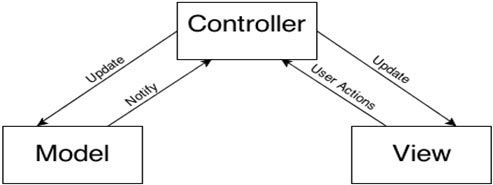
\includegraphics[width=\textwidth]{traditional_mvc1}}
\end{center}

\section{Najpoznatija okruženja (framework) za korišćenje ovog jezika i njihove karakteristike}
\label{sec:okruzenja}
\subsection{Cocoa API}
\label{sec:Cocoa}
Cocoa \cite{cocoa} je objektno-orijentisano okruženje za Mac OS X operativni sistem. Uz korišćenje Cocoa Touch dodatka za
prepoznavanje pokreta i realizaciju animacije moguća je izrada aplikacija i na iOS operativnom
sistemu koji se koristi na mobilnim uređajima kao što su iPhone, iPod i iPad.
Cocoa aplikacije se
razvijaju pomoću Xcode i Interface Builder alata, i razvijaju se u programskom jeziku Objective-C.
Pored nabrojanih alata Cocoa aplikaciju je moguće pisati u jednostavnom uređivaču teksta i
napraviti izvršnu verziju programa pomoću GCC prevodioca iz komandne linije.

\subsubsection{Istorijat razvoja Cocoa}
Cocoa je izveden iz NeXTSTEP i OPENSTEP programerskih okruženja razvijenih u NeXT-u kasnih 1980-tih. Apple je kupio NeXT u decembru 1996. godine, i postepeno je počeo da radi na Rhapsody operativnom sistemu koji je trebao da bude direktni naslednik OPENSTEP-a. Trebao je da ima emulacionu bazu za Mac OS aplikacije pod imenom Blue Box. OPENSTEP baza biblioteka i binarna podrška su nazvani Yellow Box. Rhapsody je evoluirao u Mac OS X, a Yellow Box je postao Cocoa. Kao rezultat, Cocoa klase počinju sa skraćenicom ,,NS'' (za NeXT-Sun kreaciju OPENSTEP-a): NSString, NSArray, i tako dalje.


Pre njegove sadašnje upotrebe ,,Cocoa'' je bilo ime programa koji je omogućavao deci da kreiraju multimedijalne projekte. Originalno je bila poznata kao KidSim, a sada je licencirana drugoj firmi kao Stagecast Creator. Program je prestao da se razvija u jednoj od racionalizacija koje su sprovedene nakon što se Steve Jobs vratio u Apple. Ime je ponovo upotrebljeno kako bi se izbeglo odlaganje koje bi nastalo registrovanjem novog žiga (eng.~{\em trademark}), uz saglasnost Stagecast-a da reklamira stari Cocoa pod novim imenom.


\subsection{GNUstep}
\label{GNUstep}
GNUstep \cite{objectivecandgnustep} je besplatno, objektno-orijentisano okruženje, namenjeno za različite arhitekture koje teži jednostavnosti i elegantnosti. U potpunosti je kompatibilno sa Cocoa \ref{sec:Cocoa} okruženjem. Namenjeno je kako razvijanju naprednih desktop aplikacija, tako i serverskih aplikacija. Za razliku od Cocoa moguće je pisati programe za različite operativne sistemime (Solaris, GNU/Linux, NetBSD, OpenBSD, FreeBSD, Windows). 
Osnovni jezik za razvoj je Objective-C, ali GNUstep nije ograničen samo na to (Java, Ruby, Guile, Scheme).

\subsubsection{Razvoj aplikacija}
Za razvoj scenskih komponenti aplikacije je namenjen Gorm \cite{gorm}, dok ProjectCenter \cite{projectcenter} predstavlja integrisano razvojno okruženje (eng.~{\em IDE}).   
Korisničko okruženje Etoile \cite{etoile} koje je moguće koristiti na različitim operativnim sistemima je u potpunosti implementirano koristeći GNUstep. 
  
\section{Instalacija i uputstvo za pokretanje na Linux/Windows operativnim sistemima}
\label{sec:instalacija}
\subsection{Instalacija na Linux operativnim sistemima}
\subsubsection{Instalacija neophodnih paketa}
Da bismo mogli da kompajliramo programe napisane u Objective-C, potrebno je prvo da instaliramo
par paketa. Za kompajliranje Objective-C programa koristi se GCC kompajler{\cite{gcc}, uz još par
dodataka.
Prvo što treba da uradimo je da instaliramo GCC podršku za Objective-C.

\begin{lstlisting}[frame=single]
$ sudo apt-get install gobjc
\end{lstlisting}
Zatim treba da instaliramo radno okruženje (eng.~{\em framework}) na kom se moderni Objective-C zasniva i bez kog ne bi imalo puno smisla raditi, iako je moguće.
To okruženje se zove GNUstep \cite{gnustep} i instalira se komandama:
\begin{lstlisting}[frame=single]
$ sudo apt-get install gnustep
$ sudo apt-get install gnustep-devel
\end{lstlisting}
\subsubsection{Kompajliranje}
Svaki put kada pokrenemo novu sesiju, moramo da pokrenemo skript GNUstep.sh, da bismo mogli da kompajliramo Objective-C programe.
\begin{lstlisting}[frame=single]
$ chmod +x /usr/share/GNUstep/Makefiles/GNUstep.sh
$ /usr/share/GNUstep/Makefiles/GNUstep.sh
\end{lstlisting}
Da ne bismo svaki put morali da izvršavamo taj skript, možemo da uradimo sledeće:
\begin{lstlisting}[frame=single]
$ echo /usr/share/GNUstep/Makefiles/GNUstep.sh >> ~/.bashrc
\end{lstlisting}

Na taj način, svaki put kad se pokrene nova sesija, biće izvršen GNUstep.sh i nećemo morati da brinemo.

Kao što smo već naveli, Objective-C koristi GNU-ov C kompajler, uz dodatnu
podršku.
Sem standardnih argumenata, GCC-u su potrebni i dodatni argumenti (eng.~{\em flags}), kao što su -lobjc, -lgnustep-base, itd.

Dakle ako želimo da prevedemo hello.m program, moramo da izvršimo sledeće:
\begin{lstlisting}[frame=single]
$ gcc hello.m -o hello `gnustep-config --objc-flags` -lgnustep-base -lobjc
\end{lstlisting}
Izvršavanje programa se radi uobičajeno:
\begin{lstlisting}[frame=single]
$ ./hello
\end{lstlisting}

\subsection{Instalacija na Windows operativnim sistemima}
\subsubsection{Kompajliranje i izvršavanje}
Kada smo instalirali MinGW i GNUstep, možemo da kompajliramo i izvršavamo Objective-C programe u shell okruženju, koje pokrećemo tako što otvorimo Shell program koji se nalazi u GNUstep.
Inicijalno se nalazimo u C:\\GNUstep\\home\\<username> direktorijumu.
Program ćemo kompajlirati sledećom naredbom:
\begin{lstlisting}[frame=single]
$ gcc `gnustep-config --objc-flags` -L /GNUstep/System/Library/Libraries hello.m -o hello -lgnustep-base -lobjc
\end{lstlisting}
A izvršavanje sa:
\begin{lstlisting}[frame=single]
./hello.exe
\end{lstlisting}
\section{Primer jednostavnog koda i njegovo objašnjenje}
\label{sec:primer}
Zatim, navedimo primer zanimljivog koda koji omogućava kategorije (eng.~{\em categories}). Kategorije su koncept jeyika Objective-C koji omogućava korisnu funkcionalnost dodavanja metode klasi samo za određenu upotrebu. Dakle, koristeći kategorije, možemo dodati neku metodu u klasu, ali samo za svoju aplikaciju, tako da klasa zapravo ostane ista. Svaka metoda uvedena kroz kategoriju biće dostupna svim instancama te klase (u okviru aplikacije u kojoj je dodata, naravno), kao i instancama svih klasa koje je nasleđuju. Pri izvršavanju takvih metoda nema nikakve razlike u odnosu metode iz klase napravljene na tradicionalan način.


\begin{lstlisting}[frame=single]
@interface NSString(MyAdditions)
+(NSString *)getCopyRightString;
@end

@implementation NSString(MyAdditions)

+(NSString *)getCopyRightString {
   return @"Zdravo";
}
@end
\end{lstlisting}

Sintaksa kojom se najavljuje da će biti uvedena kategorija je ista kao i kad se deklariše klasa (interface, end, između definicija), sa dodatkom imena kategorije u zagradama:

\begin{lstlisting}[frame=single]
@interface ImeKlase (ImeKategorije)

@end
\end{lstlisting}

Tu se posle znaka + navodi (u zagradama) tip, a potom ime metode koja će biti dodata klasi, a zatim se ključnim rečima implementation i end najavljuje da između njih sledi definicija nečega, u ovom slučaju gorenavedene kategorije. Tu se znakom + najavljuje dodavanje metode, a posle njenog tipa i imena u vitičastim zadradama sledi kod. Ovde smo definisali jednu jednostavnu metodu koja vraća nisku ,,Zdravo".

\section{Zaključak}
\label{sec:zakljucak}
U ovom radu su opisane najvažnije osobine i koncepti jezika. Objective-C predstavlja osnovu operativnih sistema koji su u širokoj upotrebi i kao takav će i u budućnosti zauzimati zapaženo mesto u svetu informatike. Trajanje (skoro 40 godina) svedoči o kvalitetu jezika. Rad prestavlja podstrek za dalje istraživanje mogućnosti i funkcionalnosti jezika i njegovih okruženja.  

\addcontentsline{toc}{section}{Literatura}
\appendix
\bibliography{seminarski} 
\bibliographystyle{plain}

\end{document}